{[}TOC{]}

\section{第五章
卷积神经网络(CNN)}\label{ux7b2cux4e94ux7ae0-ux5377ux79efux795eux7ecfux7f51ux7edccnn}

​
卷积神经网络是一种用来处理局部和整体相关性的计算网络结构,被应用在图像识别、自然语言处理甚至是语音识别领域,因为图像数据具有显著的局部与整体关系,其在图像识别领域的应用获得了巨大的成功。

\subsection{5.1
卷积神经网络的组成层}\label{ux5377ux79efux795eux7ecfux7f51ux7edcux7684ux7ec4ux6210ux5c42}

​
以图像分类任务为例,在表5.1所示卷积神经网络中,一般包含5种类型的网络层次结构:

​ 表5.1 卷积神经网络的组成

\begin{longtable}[]{@{}ccl@{}}
\toprule
CNN层次结构 & 输出尺寸 & 作用\tabularnewline
\midrule
\endhead
输入层 & \(W_1\times H_1\times 3\) &
卷积网络的原始输入,可以是原始或预处理后的像素矩阵\tabularnewline
卷积层 & \(W_1\times H_1\times K\) &
参数共享、局部连接,利用平移不变性从全局特征图提取局部特征\tabularnewline
激活层 & \(W_1\times H_1\times K\) &
将卷积层的输出结果进行非线性映射\tabularnewline
池化层 & \(W_2\times H_2\times K\) &
进一步筛选特征,可以有效减少后续网络层次所需的参数量\tabularnewline
全连接层 & \((W_2 \cdot H_2 \cdot K)\times C\) &
将多维特征展平为2维特征,通常低维度特征对应任务的学习目标(类别或回归值)\tabularnewline
\bottomrule
\end{longtable}

\begin{quote}
\(W_1\times H_1\times 3\)对应原始图像或经过预处理的像素值矩阵,3对应RGB图像的通道;\(K\)表示卷积层中卷积核(滤波器)的个数;\(W_2\times H_2\)
为池化后特征图的尺度,在全局池化中尺度对应\(1\times 1\);\((W_2 \cdot H_2 \cdot K)\)是将多维特征压缩到1维之后的大小,\(C\)对应的则是图像类别个数。
\end{quote}

\subsubsection{5.1.1 输入层}\label{ux8f93ux5165ux5c42}

​ 输入层(Input
Layer)通常是输入卷积神经网络的原始数据或经过预处理的数据,可以是图像识别领域中原始三维的多彩图像,也可以是音频识别领域中经过傅利叶变换的二维波形数据,甚至是自然语言处理中一维表示的句子向量。以图像分类任务为例,输入层输入的图像一般包含RGB三个通道,是一个由长宽分别为\(H\)和\(W\)组成的3维像素值矩阵\(H\times W \times 3\),卷积网络会将输入层的数据传递到一系列卷积、池化等操作进行特征提取和转化,最终由全连接层对特征进行汇总和结果输出。根据计算能力、存储大小和模型结构的不同,卷积神经网络每次可以批量处理的图像个数不尽相同,若指定输入层接收到的图像个数为\(N\),则输入层的输出数据为\(N\times H\times W\times 3\)。

\subsubsection{5.1.2 卷积层}\label{ux5377ux79efux5c42}

​ 卷积层(Convolution
Layer)通常用作对输入层输入数据进行特征提取,通过卷积核矩阵对原始数据中隐含关联性的一种抽象。卷积操作原理上其实是对两张像素矩阵进行点乘求和的数学操作,其中一个矩阵为输入的数据矩阵,另一个矩阵则为卷积核(滤波器或特征矩阵),求得的结果表示为原始图像中提取的特定局部特征。图5.1表示卷积操作过程中的不同填充策略,上半部分采用零填充,下半部分采用有效卷积(舍弃不能完整运算的边缘部分)。
​ 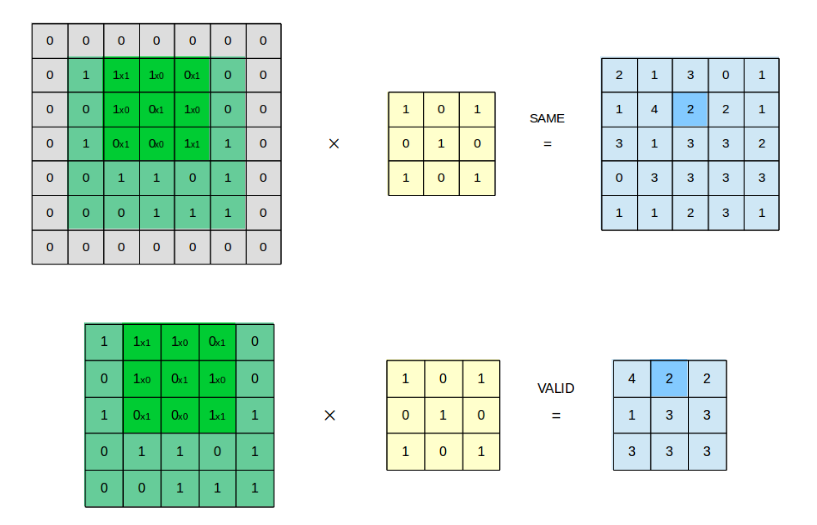
\includegraphics{img/ch5/convolution.png} ​ 图5.1 卷积操作示意图

\subsubsection{5.1.3 激活层}\label{ux6fc0ux6d3bux5c42}

​ 激活层(Activation
Layer)负责对卷积层抽取的特征进行激活,由于卷积操作是由输入矩阵与卷积核矩阵进行相差的线性变化关系,需要激活层对其进行非线性的映射。激活层主要由激活函数组成,即在卷积层输出结果的基础上嵌套一个非线性函数,让输出的特征图具有非线性关系。卷积网络中通常采用ReLU来充当激活函数(还包括tanh和sigmoid等)ReLU的函数形式如公式(5-1)所示,能够限制小于0的值为0,同时大于等于0的值保持不变。
\[
f(x)=\begin{cases}
   0 &\text{if } x<0 \\
   x &\text{if } x\ge 0
\end{cases}
\tag{5-1}
\]

\subsubsection{5.1.4 池化层}\label{ux6c60ux5316ux5c42}

​ 池化层又称为降采样层(Downsampling
Layer),作用是对感受域内的特征进行筛选,提取区域内最具代表性的特征,能够有效地降低输出特征尺度,进而减少模型所需要的参数量。按操作类型通常分为最大池化(Max
Pooling)、平均池化(Average Pooling)和求和池化(Sum
Pooling),它们分别提取感受域内最大、平均与总和的特征值作为输出,最常用的是最大池化。

\subsubsection{5.1.5 全连接层}\label{ux5168ux8fdeux63a5ux5c42}

​ 全连接层(Full Connected
Layer)负责对卷积神经网络学习提取到的特征进行汇总,将多维的特征输入映射为二维的特征输出,高维表示样本批次,低位常常对应任务目标。

\subsection{5.2
卷积在图像中有什么直观作用}\label{ux5377ux79efux5728ux56feux50cfux4e2dux6709ux4ec0ux4e48ux76f4ux89c2ux4f5cux7528}

​
在卷积神经网络中,卷积常用来提取图像的特征,但不同层次的卷积操作提取到的特征类型是不相同的,特征类型粗分如表5.2所示。
​ 表5.2 卷积提取的特征类型

\begin{longtable}[]{@{}cc@{}}
\toprule
卷积层次 & 特征类型\tabularnewline
\midrule
\endhead
浅层卷积 & 边缘特征\tabularnewline
中层卷积 & 局部特征\tabularnewline
深层卷积 & 全局特征\tabularnewline
\bottomrule
\end{longtable}

图像与不同卷积核的卷积可以用来执行边缘检测、锐化和模糊等操作。表5.3显示了应用不同类型的卷积核(滤波器)后的各种卷积图像。
​ 表5.3 一些常见卷积核的作用

\begin{longtable}[]{@{}ccc@{}}
\toprule
\begin{minipage}[b]{0.17\columnwidth}\centering\strut
卷积作用\strut
\end{minipage} & \begin{minipage}[b]{0.41\columnwidth}\centering\strut
卷积核\strut
\end{minipage} & \begin{minipage}[b]{0.34\columnwidth}\centering\strut
卷积后图像\strut
\end{minipage}\tabularnewline
\midrule
\endhead
\begin{minipage}[t]{0.17\columnwidth}\centering\strut
输出原图\strut
\end{minipage} & \begin{minipage}[t]{0.41\columnwidth}\centering\strut
\(\begin{bmatrix} 0 & 0 & 0 \\ 0 & 1 & 0 \\ 0 & 0 & 0 \end{bmatrix}\)\strut
\end{minipage} & \begin{minipage}[t]{0.34\columnwidth}\centering\strut
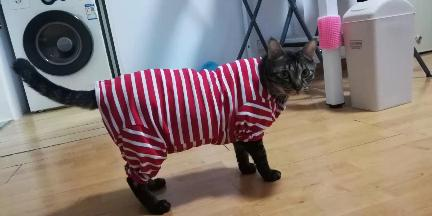
\includegraphics{./img/ch5/cat.jpg}\strut
\end{minipage}\tabularnewline
\begin{minipage}[t]{0.17\columnwidth}\centering\strut
边缘检测(突出边缘差异)\strut
\end{minipage} & \begin{minipage}[t]{0.41\columnwidth}\centering\strut
\(\begin{bmatrix} 1 & 0 & -1 \\ 0 & 0 & 0 \\ -1 & 0 & 1 \end{bmatrix}\)\strut
\end{minipage} & \begin{minipage}[t]{0.34\columnwidth}\centering\strut
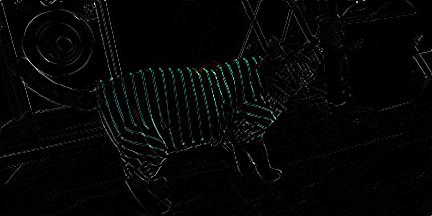
\includegraphics{./img/ch5/cat-edgeDetect.jpg}\strut
\end{minipage}\tabularnewline
\begin{minipage}[t]{0.17\columnwidth}\centering\strut
边缘检测(突出中间值)\strut
\end{minipage} & \begin{minipage}[t]{0.41\columnwidth}\centering\strut
\(\begin{bmatrix} -1 & -1 & -1 \\ -1 & 8 & -1 \\ -1 & -1 & -1 \end{bmatrix}\)\strut
\end{minipage} & \begin{minipage}[t]{0.34\columnwidth}\centering\strut
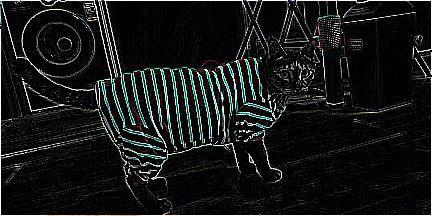
\includegraphics{./img/ch5/cat-edgeDetect-2.jpg}\strut
\end{minipage}\tabularnewline
\begin{minipage}[t]{0.17\columnwidth}\centering\strut
图像锐化\strut
\end{minipage} & \begin{minipage}[t]{0.41\columnwidth}\centering\strut
\(\begin{bmatrix} 0 & -1 & 0 \\ -1 & 5 & -1 \\ 0 & -1 & 0 \end{bmatrix}\)\strut
\end{minipage} & \begin{minipage}[t]{0.34\columnwidth}\centering\strut
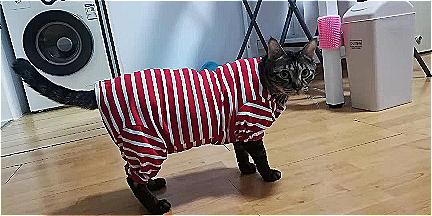
\includegraphics{./img/ch5/cat-sharpen.jpg}\strut
\end{minipage}\tabularnewline
\begin{minipage}[t]{0.17\columnwidth}\centering\strut
方块模糊\strut
\end{minipage} & \begin{minipage}[t]{0.41\columnwidth}\centering\strut
\(\begin{bmatrix} 1 & 1 & 1 \\ 1 & 1 & 1 \\ 1 & 1 & 1 \end{bmatrix} \times \frac{1}{9}\)\strut
\end{minipage} & \begin{minipage}[t]{0.34\columnwidth}\centering\strut
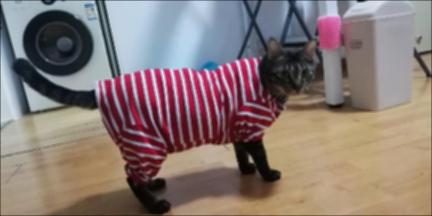
\includegraphics{./img/ch5/cat-boxblur.jpg}\strut
\end{minipage}\tabularnewline
\begin{minipage}[t]{0.17\columnwidth}\centering\strut
高斯模糊\strut
\end{minipage} & \begin{minipage}[t]{0.41\columnwidth}\centering\strut
\(\begin{bmatrix} 1 & 2 & 1 \\ 2 & 4 & 2 \\ 1 & 2 & 1 \end{bmatrix} \times \frac{1}{16}\)\strut
\end{minipage} & \begin{minipage}[t]{0.34\columnwidth}\centering\strut
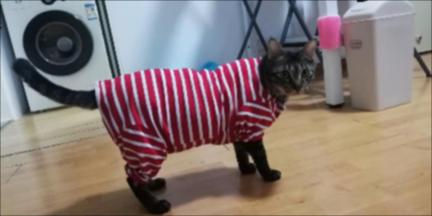
\includegraphics{./img/ch5/cat-blur-gaussian.jpg}\strut
\end{minipage}\tabularnewline
\bottomrule
\end{longtable}

\subsection{5.3
卷积层有哪些基本参数?}\label{ux5377ux79efux5c42ux6709ux54eaux4e9bux57faux672cux53c2ux6570}

​
卷积层中需要用到卷积核(滤波器或特征检测器)与图像特征矩阵进行点乘运算,利用卷积核与对应的特征感受域进行划窗式运算时,需要设定卷积核对应的大小、步长、个数以及填充的方式,如表5.4所示。

​ 表5.4 卷积层的基本参数

\begin{longtable}[]{@{}cll@{}}
\toprule
\begin{minipage}[b]{0.16\columnwidth}\centering\strut
参数名\strut
\end{minipage} & \begin{minipage}[b]{0.38\columnwidth}\raggedright\strut
作用\strut
\end{minipage} & \begin{minipage}[b]{0.38\columnwidth}\raggedright\strut
常见设置\strut
\end{minipage}\tabularnewline
\midrule
\endhead
\begin{minipage}[t]{0.16\columnwidth}\centering\strut
卷积核大小 (Kernel Size)\strut
\end{minipage} & \begin{minipage}[t]{0.38\columnwidth}\raggedright\strut
卷积核的大小定义了卷积的感受野\strut
\end{minipage} & \begin{minipage}[t]{0.38\columnwidth}\raggedright\strut
在过去常设为5,如LeNet-5;现在多设为3,通过堆叠\(3\times3\)的卷积核来达到更大的感受域\strut
\end{minipage}\tabularnewline
\begin{minipage}[t]{0.16\columnwidth}\centering\strut
卷积核步长 (Stride)\strut
\end{minipage} & \begin{minipage}[t]{0.38\columnwidth}\raggedright\strut
定义了卷积核在卷积过程中的步长\strut
\end{minipage} & \begin{minipage}[t]{0.38\columnwidth}\raggedright\strut
常见设置为1,表示滑窗距离为1,可以覆盖所有相邻位置特征的组合;当设置为更大值时相当于对特征组合降采样\strut
\end{minipage}\tabularnewline
\begin{minipage}[t]{0.16\columnwidth}\centering\strut
填充方式 (Padding)\strut
\end{minipage} & \begin{minipage}[t]{0.38\columnwidth}\raggedright\strut
在卷积核尺寸不能完美匹配输入的图像矩阵时需要进行一定的填充策略\strut
\end{minipage} & \begin{minipage}[t]{0.38\columnwidth}\raggedright\strut
设置为'SAME'表示对不足卷积核大小的边界位置进行某种填充(通常零填充)以保证卷积输出维度与与输入维度一致;当设置为'VALID'时则对不足卷积尺寸的部分进行舍弃,输出维度就无法保证与输入维度一致\strut
\end{minipage}\tabularnewline
\begin{minipage}[t]{0.16\columnwidth}\centering\strut
输入通道数 (In Channels)\strut
\end{minipage} & \begin{minipage}[t]{0.38\columnwidth}\raggedright\strut
指定卷积操作时卷积核的深度\strut
\end{minipage} & \begin{minipage}[t]{0.38\columnwidth}\raggedright\strut
默认与输入的特征矩阵通道数(深度)一致;在某些压缩模型中会采用通道分离的卷积方式\strut
\end{minipage}\tabularnewline
\begin{minipage}[t]{0.16\columnwidth}\centering\strut
输出通道数 (Out Channels)\strut
\end{minipage} & \begin{minipage}[t]{0.38\columnwidth}\raggedright\strut
指定卷积核的个数\strut
\end{minipage} & \begin{minipage}[t]{0.38\columnwidth}\raggedright\strut
若设置为与输入通道数一样的大小,可以保持输入输出维度的一致性;若采用比输入通道数更小的值,则可以减少整体网络的参数量\strut
\end{minipage}\tabularnewline
\bottomrule
\end{longtable}

\begin{quote}
卷积操作维度变换公式:

\(O_d =\begin{cases} \lceil \frac{(I_d - k_{size})+ 1)}{s}\rceil ,& \text{padding=VALID}\\ \lceil \frac{I_d}{s}\rceil,&\text{padding=SAME} \end{cases}\)

其中,\(I_d\)为输入维度,\(O_d\)为输出维度,\(k_{size}\)为卷积核大小,\(s\)为步长
\end{quote}

\subsection{5.4
卷积核有什么类型?}\label{ux5377ux79efux6838ux6709ux4ec0ux4e48ux7c7bux578b}

​
常见的卷积主要是由连续紧密的卷积核对输入的图像特征进行滑窗式点乘求和操作,除此之外还有其他类型的卷积核在不同的任务中会用到,具体分类如表5.5所示。
​ 表5.5 卷积核分类

\begin{longtable}[]{@{}ccl@{}}
\toprule
\begin{minipage}[b]{0.23\columnwidth}\centering\strut
卷积类别\strut
\end{minipage} & \begin{minipage}[b]{0.22\columnwidth}\centering\strut
示意图\strut
\end{minipage} & \begin{minipage}[b]{0.46\columnwidth}\raggedright\strut
作用\strut
\end{minipage}\tabularnewline
\midrule
\endhead
\begin{minipage}[t]{0.23\columnwidth}\centering\strut
标准卷积\strut
\end{minipage} & \begin{minipage}[t]{0.22\columnwidth}\centering\strut
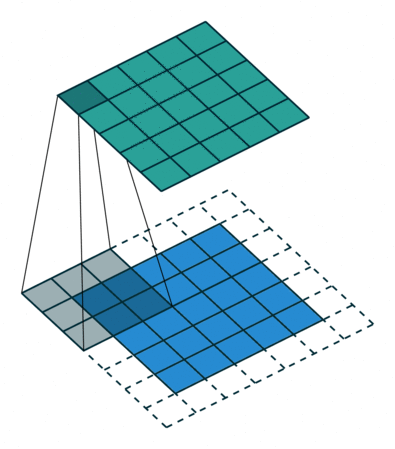
\includegraphics{./img/ch5/img7.png}\strut
\end{minipage} & \begin{minipage}[t]{0.46\columnwidth}\raggedright\strut
最常用的卷积核,连续紧密的矩阵形式可以提取图像区域中的相邻像素之间的关联关系,\(3\times3\)的卷积核可以获得\(3\times3\)像素范围的感受视野\strut
\end{minipage}\tabularnewline
\begin{minipage}[t]{0.23\columnwidth}\centering\strut
扩张卷积(带孔卷积或空洞卷积)\strut
\end{minipage} & \begin{minipage}[t]{0.22\columnwidth}\centering\strut
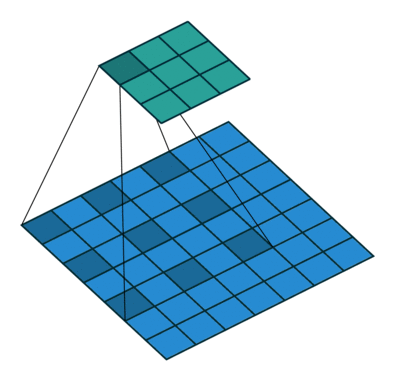
\includegraphics{./img/ch5/img8.png}\strut
\end{minipage} & \begin{minipage}[t]{0.46\columnwidth}\raggedright\strut
引入一个称作扩张率(Dilation
Rate)的参数,使同样尺寸的卷积核可以获得更大的感受视野,相应的在相同感受视野的前提下比普通卷积采用更少的参数。同样是\(3\times3\)的卷积核尺寸,扩张卷积可以提取\(5\times5\)范围的区域特征,在实时图像分割领域广泛应用\strut
\end{minipage}\tabularnewline
\begin{minipage}[t]{0.23\columnwidth}\centering\strut
转置卷积\strut
\end{minipage} & \begin{minipage}[t]{0.22\columnwidth}\centering\strut
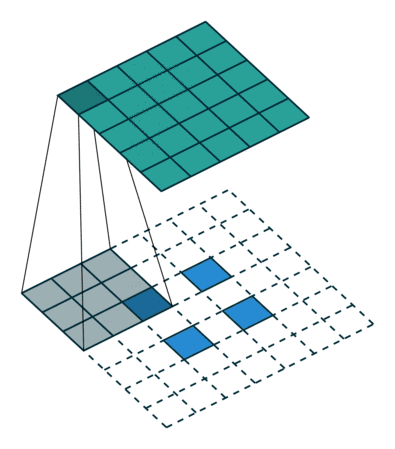
\includegraphics{./img/ch5/img10.png}\strut
\end{minipage} & \begin{minipage}[t]{0.46\columnwidth}\raggedright\strut
先对原始特征矩阵进行填充使其维度扩大到适配卷积目标输出维度,然后进行普通的卷积操作的一个过程,其输入到输出的维度变换关系恰好与普通卷积的变换关系相反,但这个变换并不是真正的逆变换操作,通常称为转置卷积(Transpose
Convolution)而不是反卷积(Deconvolution)。转置卷积常见于目标检测领域中对小目标的检测和图像分割领域还原输入图像尺度。\strut
\end{minipage}\tabularnewline
\begin{minipage}[t]{0.23\columnwidth}\centering\strut
可分离卷积\strut
\end{minipage} & \begin{minipage}[t]{0.22\columnwidth}\centering\strut
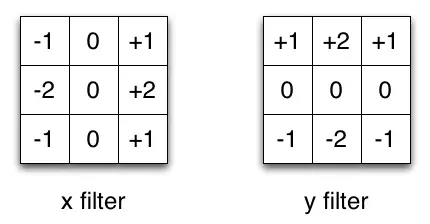
\includegraphics{./img/ch5/img11.png}\strut
\end{minipage} & \begin{minipage}[t]{0.46\columnwidth}\raggedright\strut
标准的卷积操作是同时对原始图像\(H\times W\times C\)三个方向的卷积运算,假设有\(K\)个相同尺寸的卷积核,这样的卷积操作需要用到的参数为\(H\times W\times C\times K\)个;若将长宽与深度方向的卷积操作分离出变为\(H\times W\)与\(C\)的两步卷积操作,则同样的卷积核个数\(K\),只需要\((H\times W + C)\times K\)个参数,便可得到同样的输出尺度。可分离卷积(Seperable
Convolution)通常应用在模型压缩或一些轻量的卷积神经网络中,如MobileNet\(^{[1]}\)、Xception\(^{[2]}\)等\strut
\end{minipage}\tabularnewline
\bottomrule
\end{longtable}

\subsection{5.5
二维卷积与三维卷积有什么区别?}\label{ux4e8cux7ef4ux5377ux79efux4e0eux4e09ux7ef4ux5377ux79efux6709ux4ec0ux4e48ux533aux522b}

\begin{itemize}
\tightlist
\item
  \textbf{二维卷积}
  二维卷积操作如图5.3所示,为了更直观的说明,分别展示在单通道和多通道输入中,对单个通道输出的卷积操作。在单通道输入的情况下,若输入卷积核尺寸为
  \((k_h, k_w, 1)​\),卷积核在输入图像的空间维度上进行滑窗操作,每次滑窗和
  \((k_h, k_w)​\)窗口内的值进行卷积操作,得到输出图像中的一个值。在多通道输入的情况下,假定输入图像特征通道数为3,卷积核尺寸则为\((k_h, k_w, 3)​\),每次滑窗与3个通道上的\((k_h, k_w)​\)窗口内的所有值进行卷积操作,得到输出图像中的一个值。
\end{itemize}

\begin{figure}
\centering
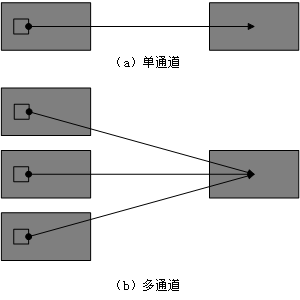
\includegraphics{./img/ch5/5.6.1.png}
\caption{image}
\end{figure}

\begin{itemize}
\tightlist
\item
  \textbf{三维卷积}
  3D卷积操作如图所示,同样分为单通道和多通道,且假定只使用1个卷积核,即输出图像仅有一个通道。对于单通道输入,与2D卷积不同之处在于,输入图像多了一个深度(depth)维度,卷积核也多了一个\(k_d​\)维度,因此3D卷积核的尺寸为\((k_h, k_w, k_d)​\),每次滑窗与\((k_h, k_w, k_d)​\)窗口内的值进行相关操作,得到输出3D图像中的一个值。对于多通道输入,则与2D卷积的操作一样,每次滑窗与3个channels上的\((k_h, k_w, k_d)​\)窗口内的所有值进行相关操作,得到输出3D图像中的一个值。
\end{itemize}

\begin{figure}
\centering
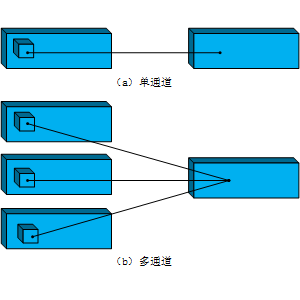
\includegraphics{./img/ch5/5.6.2.png}
\caption{image}
\end{figure}

\subsection{5.7
有哪些池化方法?}\label{ux6709ux54eaux4e9bux6c60ux5316ux65b9ux6cd5}

​
池化操作通常也叫做子采样(Subsampling)或降采样(Downsampling),在构建卷积神经网络时,往往会用在卷积层之后,通过池化来降低卷积层输出的特征维度,有效减少网络参数的同时还可以防止过拟合现象。池化操作可以降低图像维度的原因,本质上是因为图像具有一种``静态性''的属性,这个意思是说在一个图像区域有用的特征极有可能在另一个区域同样有用。因此,为了描述一个大的图像,很直观的想法就是对不同位置的特征进行聚合统计。例如,可以计算图像在固定区域上特征的平均值
(或最大值)来代表这个区域的特征。 ​ 表5.6 池化分类

\begin{longtable}[]{@{}ccl@{}}
\toprule
\begin{minipage}[b]{0.26\columnwidth}\centering\strut
池化类型\strut
\end{minipage} & \begin{minipage}[b]{0.29\columnwidth}\centering\strut
示意图\strut
\end{minipage} & \begin{minipage}[b]{0.36\columnwidth}\raggedright\strut
作用\strut
\end{minipage}\tabularnewline
\midrule
\endhead
\begin{minipage}[t]{0.26\columnwidth}\centering\strut
一般池化(General Pooling)\strut
\end{minipage} & \begin{minipage}[t]{0.29\columnwidth}\centering\strut
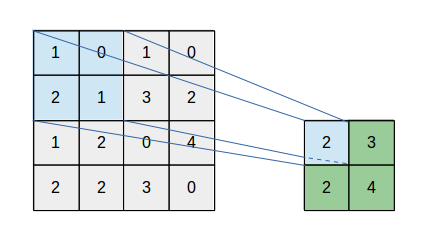
\includegraphics{./img/ch5/general_pooling.png}\strut
\end{minipage} & \begin{minipage}[t]{0.36\columnwidth}\raggedright\strut
通常包括最大池化(Max Pooling)和平均池化(Mean
Pooling)。以最大池化为例,池化范围\((2\times2)\)和滑窗步长\((stride=2)\)
相同,仅提取一次相同区域的范化特征。\strut
\end{minipage}\tabularnewline
\begin{minipage}[t]{0.26\columnwidth}\centering\strut
重叠池化(Overlapping Pooling)\strut
\end{minipage} & \begin{minipage}[t]{0.29\columnwidth}\centering\strut
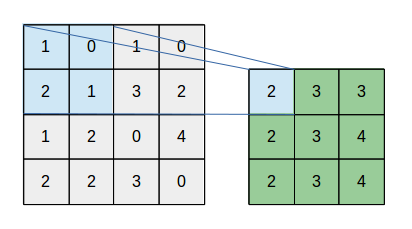
\includegraphics{./img/ch5/overlap_pooling.png}\strut
\end{minipage} & \begin{minipage}[t]{0.36\columnwidth}\raggedright\strut
与一般池化操作相同,但是池化范围\(P_{size}\)与滑窗步长\(stride\)关系为\(P_{size}>stride\),同一区域内的像素特征可以参与多次滑窗提取,得到的特征表达能力更强,但计算量更大。\strut
\end{minipage}\tabularnewline
\begin{minipage}[t]{0.26\columnwidth}\centering\strut
空间金字塔池化\(^*\)(Spatial Pyramid Pooling)\strut
\end{minipage} & \begin{minipage}[t]{0.29\columnwidth}\centering\strut
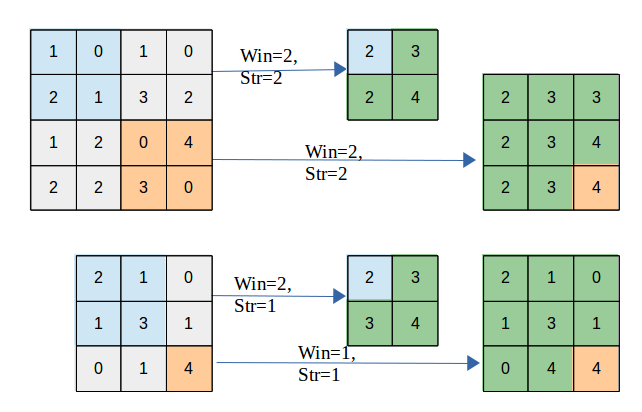
\includegraphics{./img/ch5/spatial_pooling.png}\strut
\end{minipage} & \begin{minipage}[t]{0.36\columnwidth}\raggedright\strut
在进行多尺度目标的训练时,卷积层允许输入的图像特征尺度是可变的,紧接的池化层若采用一般的池化方法会使得不同的输入特征输出相应变化尺度的特征,而卷积神经网络中最后的全连接层则无法对可变尺度进行运算,因此需要对不同尺度的输出特征采样到相同输出尺度。\strut
\end{minipage}\tabularnewline
\bottomrule
\end{longtable}

\begin{quote}
SPPNet\(^{[3]}\)就引入了空间池化的组合,对不同输出尺度采用不同的滑窗大小和步长以确保输出尺度相同\((win_{size}=\lceil \frac{in}{out}\rceil; stride=\lfloor \frac{in}{out}\rfloor; )\),同时用如金字塔式叠加的多种池化尺度组合,以提取更加丰富的图像特征。常用于多尺度训练和目标检测中的区域提议网络(Region
Proposal Network)的兴趣区域(Region of Interest)提取
\end{quote}

\subsection{\texorpdfstring{5.8
\(1\times1\)卷积作用?}{5.8 1\textbackslash{}times1卷积作用?}}\label{times1ux5377ux79efux4f5cux7528}

​ NIN(Network in
Network)\(^{[4]}​\)是第一篇探索\(1\times1​\)卷积核的论文,这篇论文通过在卷积层中使用MLP替代传统线性的卷积核,使单层卷积层内具有非线性映射的能力,也因其网络结构中嵌套MLP子网络而得名NIN。NIN对不同通道的特征整合到MLP自网络中,让不同通道的特征能够交互整合,使通道之间的信息得以流通,其中的MLP子网络恰恰可以用\(1\times1​\)的卷积进行代替。

​
GoogLeNet\(^{[5]}​\)则采用\(1\times1​\)卷积核来减少模型的参数量。在原始版本的Inception模块中,由于每一层网络采用了更多的卷积核,大大增加了模型的参数量。此时在每一个较大卷积核的卷积层前引入\(1\times1​\)卷积,可以通过分离通道与宽高卷积来减少模型参数量。以图5.2为例,在不考虑参数偏置项的情况下,若输入和输出的通道数为\(C_1=16​\),则左半边网络模块所需的参数为\((1\times1+3\times3+5\times5+0)\times C_1\times C_1=8960​\);假定右半边网络模块采用的\(1\times1​\)卷积通道数为\(C_2=8​\)\((满足C_1>C_2)​\),则右半部分的网络结构所需参数量为\((1\times1\times (3C_1+C_2)+3\times3\times C_2 +5\times5\times C_2)\times C_1=5248​\)
,可以在不改变模型表达能力的前提下大大减少所使用的参数量。

\begin{figure}
\centering
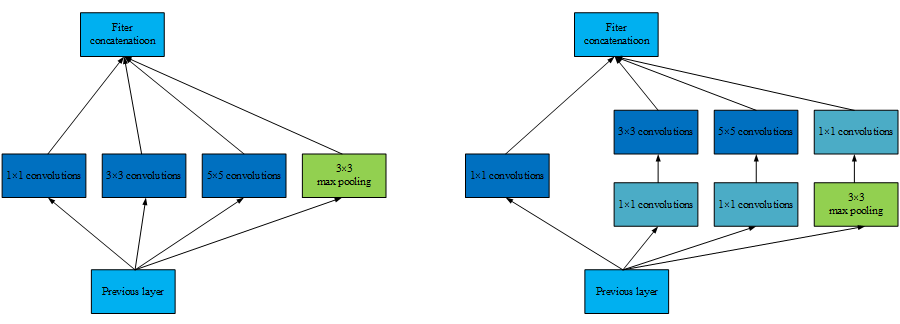
\includegraphics{./img/ch5/5.8-1.png}
\caption{image}
\end{figure}

​ 图5.2 Inception模块

综上所述,\(1\times 1​\)卷积的作用主要为以下两点:

\begin{itemize}
\tightlist
\item
  实现信息的跨通道交互和整合。
\item
  对卷积核通道数进行降维和升维,减小参数量。
\end{itemize}

\subsection{5.9
卷积层和池化层有什么区别?}\label{ux5377ux79efux5c42ux548cux6c60ux5316ux5c42ux6709ux4ec0ux4e48ux533aux522b}

​
卷积层核池化层在结构上具有一定的相似性,都是对感受域内的特征进行提取,并且根据步长设置获取到不同维度的输出,但是其内在操作是有本质区别的,如表5.7所示。

\begin{longtable}[]{@{}ccc@{}}
\toprule
& 卷积层 & 池化层\tabularnewline
\midrule
\endhead
\textbf{结构} & 零填充时输出维度不变,而通道数改变 &
通常特征维度会降低,通道数不变\tabularnewline
\textbf{稳定性} & 输入特征发生细微改变时,输出结果会改变 &
感受域内的细微变化不影响输出结果\tabularnewline
\textbf{作用} & 感受域内提取局部关联特征 &
感受域内提取泛化特征,降低维度\tabularnewline
\textbf{参数量} & 与卷积核尺寸、卷积核个数相关 &
不引入额外参数\tabularnewline
\bottomrule
\end{longtable}

\subsection{5.10
卷积核是否一定越大越好?}\label{ux5377ux79efux6838ux662fux5426ux4e00ux5b9aux8d8aux5927ux8d8aux597d}

​
在早期的卷积神经网络中(如LeNet-5、AlexNet),用到了一些较大的卷积核(\(11\times11\)和\(5\times 5\)),受限于当时的计算能力和模型结构的设计,无法将网络叠加得很深,因此卷积网络中的卷积层需要设置较大的卷积核以获取更大的感受域。但是这种大卷积核反而会导致计算量大幅增加,不利于训练更深层的模型,相应的计算性能也会降低。后来的卷积神经网络(VGG、GoogLeNet等),发现通过堆叠2个\(3\times 3\)卷积核可以获得与\(5\times 5\)卷积核相同的感受视野,同时参数量会更少(\(3×3×2+1\)
\textless{} \$
5×5×1+1\$),\(3\times 3\)卷积核被广泛应用在许多卷积神经网络中。因此可以认为,在大多数情况下通过堆叠较小的卷积核比直接采用单个更大的卷积核会更加有效。

​
但是,这并不是表示更大的卷积核就没有作用,在某些领域应用卷积神经网络时仍然可以采用较大的卷积核。譬如在自然语言处理领域,由于文本内容不像图像数据可以对特征进行很深层的抽象,往往在该领域的特征提取只需要较浅层的神经网络即可。在将卷积神经网络应用在自然语言处理领域时,通常都是较为浅层的卷积层组成,但是文本特征有时又需要有较广的感受域让模型能够组合更多的特征(如词组和字符),此时直接采用较大的卷积核将是更好的选择。

​
综上所述,卷积核的大小并没有绝对的优劣,需要视具体的应用场景而定,但是极大和极小的卷积核都是不合适的,单独的\(1\times 1\)极小卷积核只能用作分离卷积而不能对输入的原始特征进行有效的组合,极大的卷积核通常会组合过多的无意义特征从而浪费了大量的计算资源。

\subsection{5.11
每层卷积是否只能用一种尺寸的卷积核?}\label{ux6bcfux5c42ux5377ux79efux662fux5426ux53eaux80fdux7528ux4e00ux79cdux5c3aux5bf8ux7684ux5377ux79efux6838}

​
经典的神经网络一般都属于层叠式网络,每层仅用一个尺寸的卷积核,如VGG结构中使用了大量的\(3×3\)卷积层。事实上,同一层特征图可以分别使用多个不同尺寸的卷积核,以获得不同尺度的特征,再把这些特征结合起来,得到的特征往往比使用单一卷积核的要好,如GoogLeNet、Inception系列的网络,均是每层使用了多个卷积核结构。如图5.3所示,输入的特征在同一层分别经过\(1×1\)、\(3×3\)和\(5×5\)三种不同尺寸的卷积核,再将分别得到的特征进行整合,得到的新特征可以看作不同感受域提取的特征组合,相比于单一卷积核会有更强的表达能力。

\begin{figure}
\centering
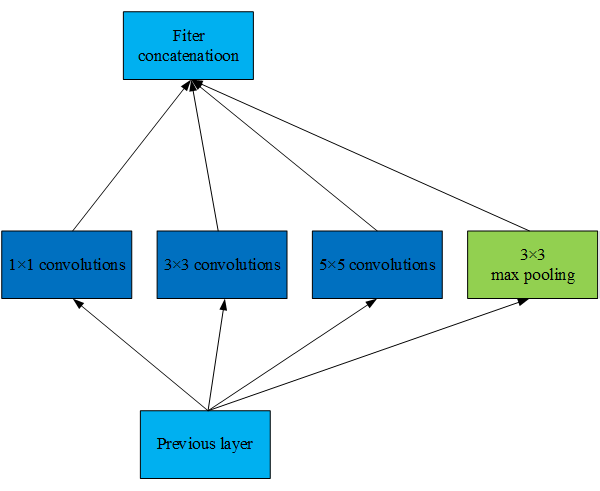
\includegraphics{./img/ch5/5.11-1.png}
\caption{image}
\end{figure}

​ 图5.3 Inception模块结构

\subsection{5.12
怎样才能减少卷积层参数量?}\label{ux600eux6837ux624dux80fdux51cfux5c11ux5377ux79efux5c42ux53c2ux6570ux91cf}

减少卷积层参数量的方法可以简要地归为以下几点:

\begin{itemize}
\tightlist
\item
  使用堆叠小卷积核代替大卷积核:VGG网络中2个\(3\times 3\)的卷积核可以代替1个\(5\times 5\)的卷积核
\item
  使用分离卷积操作:将原本\(K\times K\times C\)的卷积操作分离为\(K\times K\times 1\)和\(1\times1\times C\)的两部分操作
\item
  添加\(1\times 1\)的卷积操作:与分离卷积类似,但是通道数可变,在\(K\times K\times C_1\)卷积前添加\(1\times1\times C_2\)的卷积核(满足\(C_2 <C_1\))
\item
  在卷积层前使用池化操作:池化可以降低卷积层的输入特征维度
\end{itemize}

\subsection{5.13
在进行卷积操作时,必须同时考虑通道和区域吗?}\label{ux5728ux8fdbux884cux5377ux79efux64cdux4f5cux65f6ux5fc5ux987bux540cux65f6ux8003ux8651ux901aux9053ux548cux533aux57dfux5417}

​ 标准卷积中,采用区域与通道同时处理的操作,如下图所示:

\begin{figure}
\centering
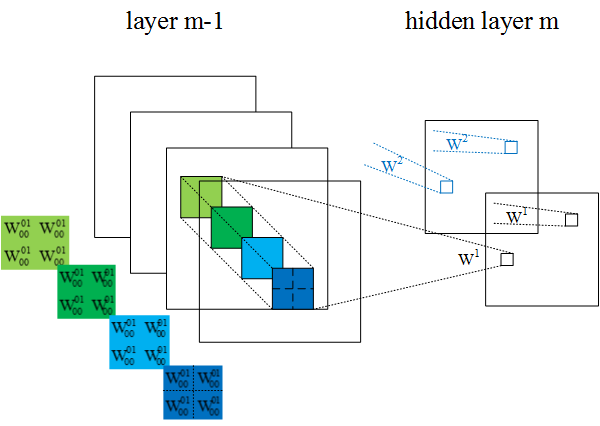
\includegraphics{./img/ch5/5.13-1.png}
\caption{image}
\end{figure}

​
这样做可以简化卷积层内部的结构,每一个输出的特征像素都由所有通道的同一个区域提取而来。

​
但是这种方式缺乏灵活性,并且在深层的网络结构中使得运算变得相对低效,更为灵活的方式是使区域和通道的卷积分离开来,通道分离(深度分离)卷积网络由此诞生。如下图所示,Xception网络可解决上述问题。

\begin{figure}
\centering
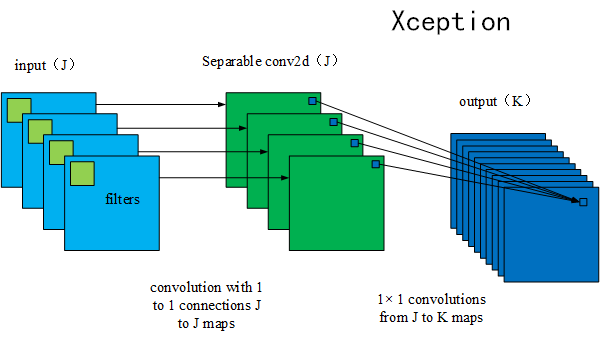
\includegraphics{./img/ch5/5.13-2.png}
\caption{image}
\end{figure}

​
我们首先对每一个通道进行各自的卷积操作,有多少个通道就有多少个过滤器。得到新的通道特征矩阵之后,再对这批新通道特征进行标准的\(1×1​\)跨通道卷积操作。

\subsection{5.14
采用宽卷积的好处有什么?}\label{ux91c7ux7528ux5bbdux5377ux79efux7684ux597dux5904ux6709ux4ec0ux4e48}

​
宽卷积对应的是窄卷积,实际上并不是卷积操作的类型,指的是卷积过程中的填充方法,对应的是'SAME'填充和'VALID'填充。'SAME'填充通常采用零填充的方式对卷积核不满足整除条件的输入特征进行补全,以使卷积层的输出维度保持与输入特征维度一致;'VALID'填充的方式则相反,实际并不进行任何填充,在输入特征边缘位置若不足以进行卷积操作,则对边缘信息进行舍弃,因此在步长为1的情况下该填充方式的卷积层输出特征维度可能会略小于输入特征的维度。此外,由于前一种方式通过补零来进行完整的卷积操作,可以有效地保留原始的输入特征信息。

​
比如下图左部分为窄卷积。注意到越在边缘的位置被卷积的次数越少。宽卷积可以看作在卷积之前在边缘用0补充,常见有两种情况,一个是全补充,如下图右部分,这样输出大于输入的维度。另一种常用的方法是补充一一部分0值,使得输出和输入的维度一致。

\begin{figure}
\centering
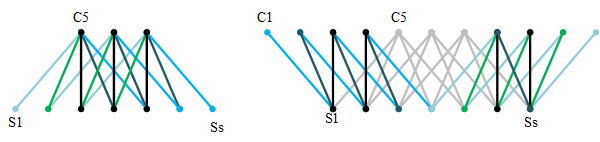
\includegraphics{./img/ch5/5.14.1.png}
\caption{image}
\end{figure}

\subsection{5.15
理解转置卷积与棋盘效应}\label{ux7406ux89e3ux8f6cux7f6eux5377ux79efux4e0eux68cbux76d8ux6548ux5e94}

\subsubsection{5.15.1 标准卷积}\label{ux6807ux51c6ux5377ux79ef}

在理解转置卷积之前,需要先理解标准卷积的运算方式。

首先给出一个输入输出结果

\begin{figure}
\centering
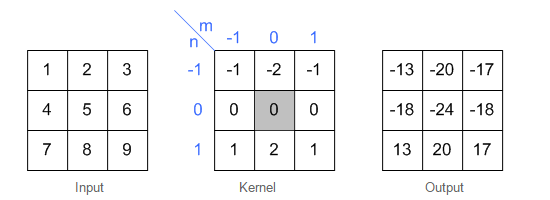
\includegraphics{./img/ch5/img32.png}
\caption{image}
\end{figure}

那是怎样计算的呢?

卷积的时候需要对卷积核进行180的旋转,同时卷积核中心与需计算的图像像素对齐,输出结构为中心对齐像素的一个新的像素值,计算例子如下:

\begin{figure}
\centering
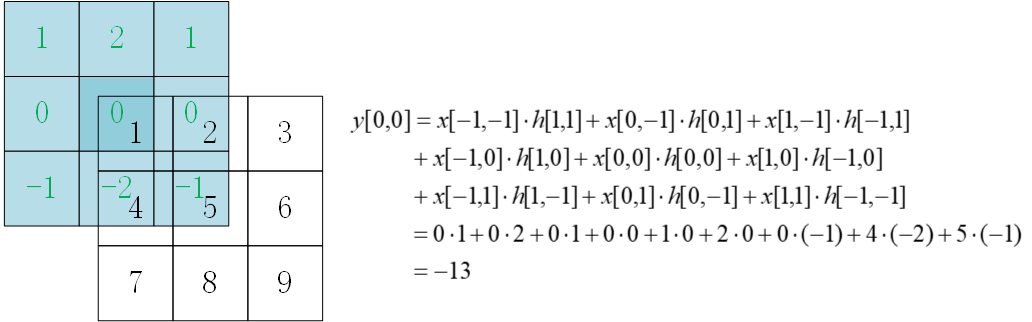
\includegraphics{./img/ch5/5.19.1-2.png}
\caption{image}
\end{figure}

这样计算出左上角(即第一行第一列)像素的卷积后像素值。

给出一个更直观的例子,从左到右看,原像素经过卷积由1变成-8。

\begin{figure}
\centering
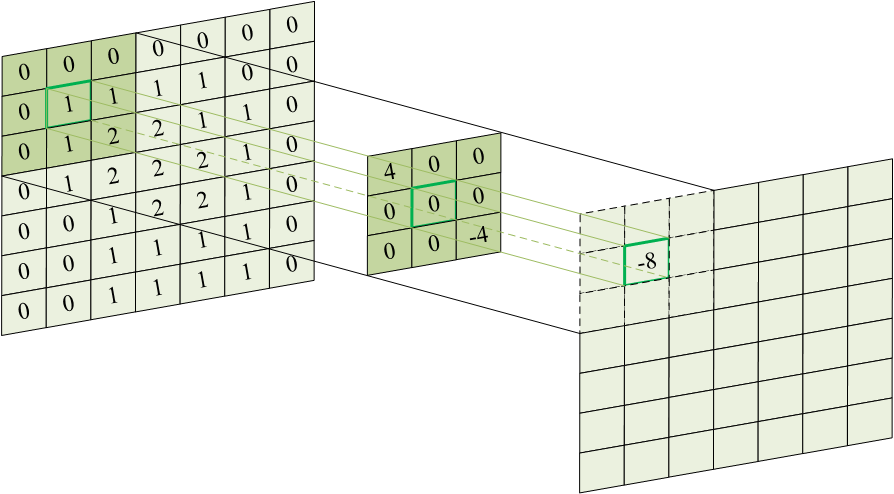
\includegraphics{./img/ch5/5.19.1-3.png}
\caption{image}
\end{figure}

通过滑动卷积核,就可以得到整张图片的卷积结果。

\subsubsection{5.15.2 转置卷积}\label{ux8f6cux7f6eux5377ux79ef}

图像的deconvolution过程如下:

\begin{figure}
\centering
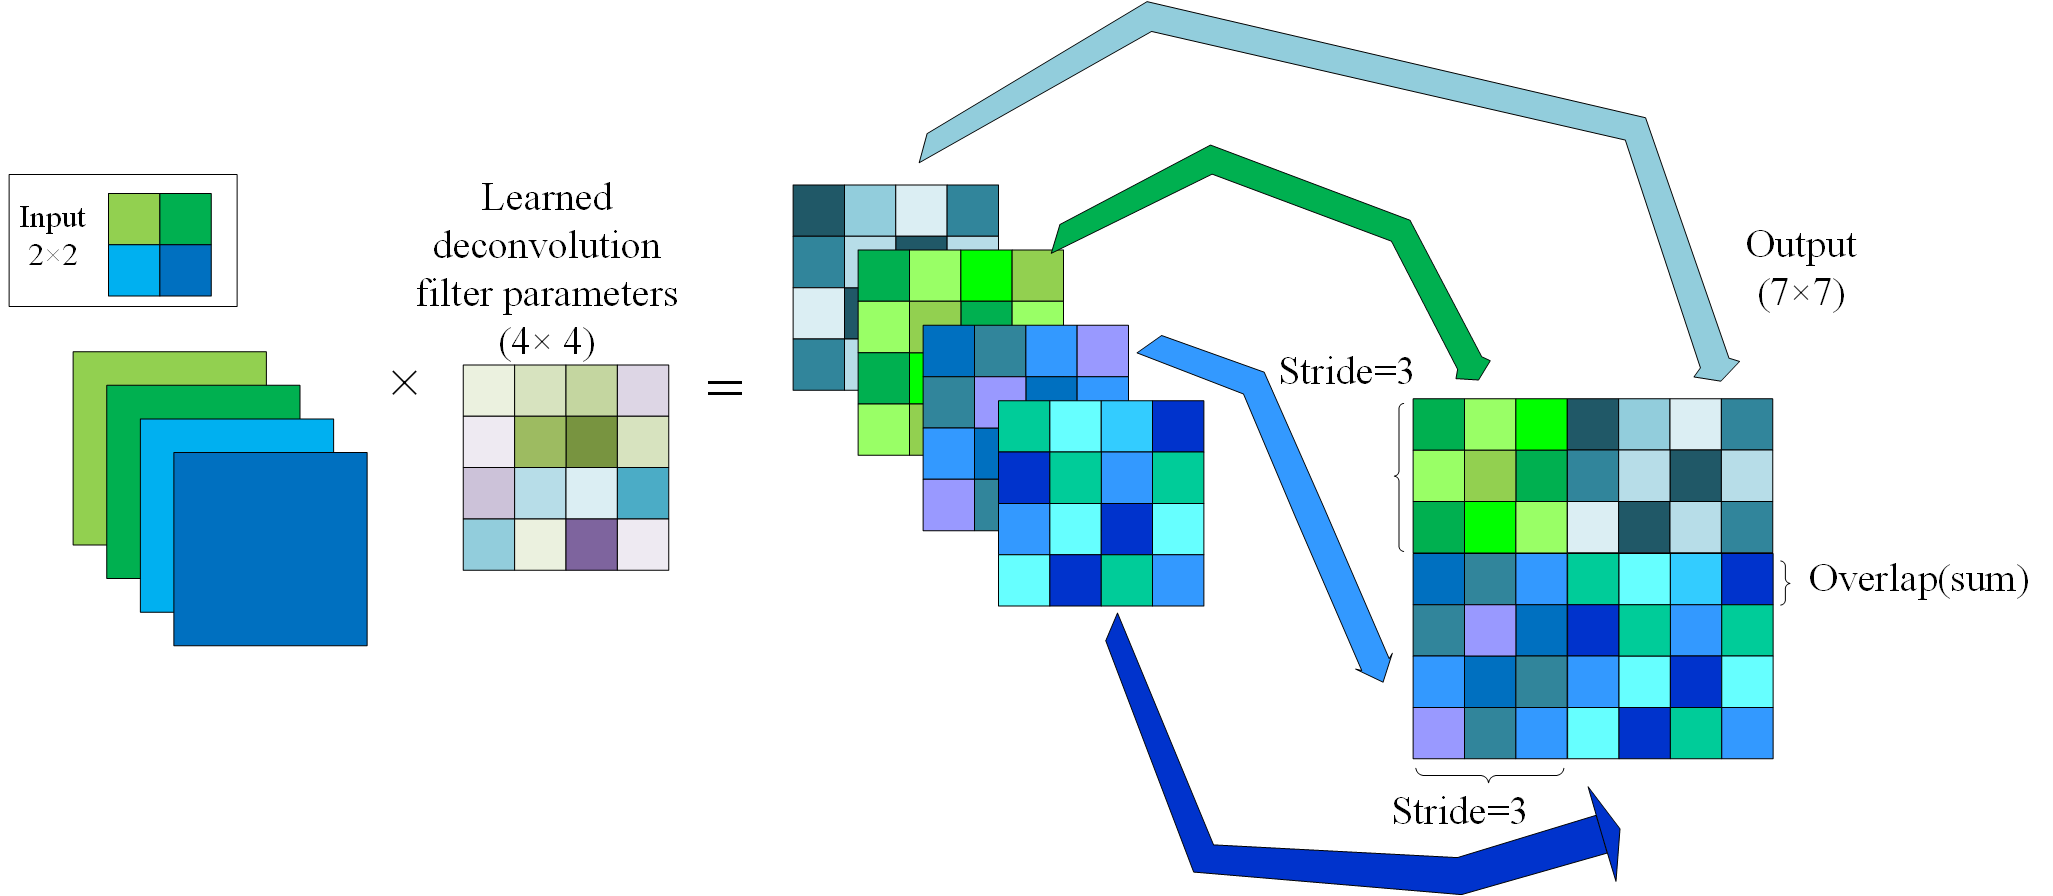
\includegraphics{./img/ch5/5.19.2-5.png}
\caption{image}
\end{figure}

输入:2x2, 卷积核:4x4, 滑动步长:3, 输出:7x7

过程如下:

\begin{enumerate}
\def\labelenumi{\arabic{enumi}.}
\item
  输入图片每个像素进行一次full卷积,根据full卷积大小计算可以知道每个像素的卷积后大小为
  1+4-1=4, 即4x4大小的特征图,输入有4个像素所以4个4x4的特征图
\item
  将4个特征图进行步长为3的相加;
  输出的位置和输入的位置相同。步长为3是指每隔3个像素进行相加,重叠部分进行相加,即输出的第1行第4列是由红色特阵图的第一行第四列与绿色特征图的第一行第一列相加得到,其他如此类推。
\end{enumerate}

可以看出翻卷积的大小是由卷积核大小与滑动步长决定, in是输入大小,
k是卷积核大小, s是滑动步长, out是输出大小 得到 out = (in - 1) * s + k
上图过程就是, (2 - 1) * 3 + 4 = 7。

\subsubsection{5.15.3 棋盘效应}\label{ux68cbux76d8ux6548ux5e94}

\subsection{5.16
卷积神经网络的参数设置}\label{ux5377ux79efux795eux7ecfux7f51ux7edcux7684ux53c2ux6570ux8bbeux7f6e}

​
卷积神经网络中常见的参数在其他类型的神经网络中也是类似的,但是参数的设置还得结合具体的任务才能设置在合理的范围,具体的参数列表如表XX所示。
​ 表XX 卷积神经网络常见参数

\begin{longtable}[]{@{}ccl@{}}
\toprule
\begin{minipage}[b]{0.09\columnwidth}\centering\strut
参数名\strut
\end{minipage} & \begin{minipage}[b]{0.10\columnwidth}\centering\strut
常见设置\strut
\end{minipage} & \begin{minipage}[b]{0.08\columnwidth}\raggedright\strut
参数说明\strut
\end{minipage}\tabularnewline
\midrule
\endhead
\begin{minipage}[t]{0.09\columnwidth}\centering\strut
学习率(Learning Rate)\strut
\end{minipage} & \begin{minipage}[t]{0.10\columnwidth}\centering\strut
\(0-1\)\strut
\end{minipage} & \begin{minipage}[t]{0.08\columnwidth}\raggedright\strut
反向传播网络中更新权值矩阵的步长,在一些常见的网络中会在固定迭代次数或模型不再收敛后对学习率进行指数下降(如\(lr=lr\times 0.1\))。当学习率越大计算误差对权值矩阵的影响越大,容易在某个局部最优解附近震荡;越小的学习率对网络权值的更新越精细,但是需要花费更多的时间去迭代\strut
\end{minipage}\tabularnewline
\begin{minipage}[t]{0.09\columnwidth}\centering\strut
批次大小(Batch Size)\strut
\end{minipage} & \begin{minipage}[t]{0.10\columnwidth}\centering\strut
\(1-N\)\strut
\end{minipage} & \begin{minipage}[t]{0.08\columnwidth}\raggedright\strut
批次大小指定一次性流入模型的数据样本个数,根据任务和计算性能限制判断实际取值,在一些图像任务中往往由于计算性能和存储容量限制只能选取较小的值。在相同迭代次数的前提下,数值越大模型越稳定,泛化能力越强,损失值曲线越平滑,模型也更快地收敛,但是每次迭代需要花费更多的时间\strut
\end{minipage}\tabularnewline
\begin{minipage}[t]{0.09\columnwidth}\centering\strut
数据轮次(Epoch)\strut
\end{minipage} & \begin{minipage}[t]{0.10\columnwidth}\centering\strut
\(1-N\)\strut
\end{minipage} & \begin{minipage}[t]{0.08\columnwidth}\raggedright\strut
数据轮次指定所有训练数据在模型中训练的次数,根据数据集规模和分布情况会设置为不同的值。当模型较为简单或训练数据规模较小时,通常轮次不宜过高,否则模型容易过拟合;模型较为复杂或训练数据规模足够大时,可适当提高数据的训练轮次。\strut
\end{minipage}\tabularnewline
\begin{minipage}[t]{0.09\columnwidth}\centering\strut
权重衰减系数(Weight Decay)\strut
\end{minipage} & \begin{minipage}[t]{0.10\columnwidth}\centering\strut
\(0-0.001\)\strut
\end{minipage} & \begin{minipage}[t]{0.08\columnwidth}\raggedright\strut
模型训练过程中反向传播权值更新的权重衰减值\strut
\end{minipage}\tabularnewline
\bottomrule
\end{longtable}

\subsection{5.17
提高卷积神经网络的泛化能力}\label{ux63d0ux9ad8ux5377ux79efux795eux7ecfux7f51ux7edcux7684ux6cdbux5316ux80fdux529b}

​
卷积神经网络与其他类型的神经网络类似,在采用反向传播进行训练的过程中比较依赖输入的数据分布,当数据分布较为极端的情况下容易导致模型欠拟合或过拟合,表XX记录了提高卷积网络泛化能力的方法。
​ 表XX 提高卷积网络化能力的方法

\begin{longtable}[]{@{}cl@{}}
\toprule
\begin{minipage}[b]{0.08\columnwidth}\centering\strut
方法\strut
\end{minipage} & \begin{minipage}[b]{0.07\columnwidth}\raggedright\strut
说明\strut
\end{minipage}\tabularnewline
\midrule
\endhead
\begin{minipage}[t]{0.08\columnwidth}\centering\strut
使用更多数据\strut
\end{minipage} & \begin{minipage}[t]{0.07\columnwidth}\raggedright\strut
在有条件的前提下,尽可能多地获取训练数据是最理想的方法,更多的数据可以让模型得到充分的学习,也更容易提高泛化能力\strut
\end{minipage}\tabularnewline
\begin{minipage}[t]{0.08\columnwidth}\centering\strut
使用更大批次\strut
\end{minipage} & \begin{minipage}[t]{0.07\columnwidth}\raggedright\strut
在相同迭代次数和学习率的条件下,每批次采用更多的数据将有助于模型更好的学习到正确的模式,模型输出结果也会更加稳定\strut
\end{minipage}\tabularnewline
\begin{minipage}[t]{0.08\columnwidth}\centering\strut
调整数据分布\strut
\end{minipage} & \begin{minipage}[t]{0.07\columnwidth}\raggedright\strut
大多数场景下的数据分布是不均匀的,模型过多地学习某类数据容易导致其输出结果偏向于该类型的数据,此时通过调整输入的数据分布可以一定程度提高泛化能力\strut
\end{minipage}\tabularnewline
\begin{minipage}[t]{0.08\columnwidth}\centering\strut
调整目标函数\strut
\end{minipage} & \begin{minipage}[t]{0.07\columnwidth}\raggedright\strut
在某些情况下,目标函数的选择会影响模型的泛化能力,如目标函数\$f(y,y')=\strut
\end{minipage}\tabularnewline
\begin{minipage}[t]{0.08\columnwidth}\centering\strut
调整网络结构\strut
\end{minipage} & \begin{minipage}[t]{0.07\columnwidth}\raggedright\strut
在浅层卷积神经网络中,参数量较少往往使模型的泛化能力不足而导致欠拟合,此时通过叠加卷积层可以有效地增加网络参数,提高模型表达能力;在深层卷积网络中,若没有充足的训练数据则容易导致模型过拟合,此时通过简化网络结构减少卷积层数可以起到提高模型泛化能力的作用\strut
\end{minipage}\tabularnewline
\begin{minipage}[t]{0.08\columnwidth}\centering\strut
数据增强\strut
\end{minipage} & \begin{minipage}[t]{0.07\columnwidth}\raggedright\strut
数据增强又叫数据增广,在有限数据的前提下通过平移、旋转、加噪声等一些列变换来增加训练数据,同类数据的表现形式也变得更多样,有助于模型提高泛化能力,需要注意的是数据变化应尽可能不破坏元数数据的主体特征(如在图像分类任务中对图像进行裁剪时不能将分类主体目标裁出边界)。\strut
\end{minipage}\tabularnewline
\begin{minipage}[t]{0.08\columnwidth}\centering\strut
权值正则化\strut
\end{minipage} & \begin{minipage}[t]{0.07\columnwidth}\raggedright\strut
权值正则化就是通常意义上的正则化,一般是在损失函数中添加一项权重矩阵的正则项作为惩罚项,用来惩罚损失值较小时网络权重过大的情况,此时往往是网络权值过拟合了数据样本(如\(Loss=f(WX+b,y')+\frac{\lambda}{\eta}\sum{|W|}\))。\strut
\end{minipage}\tabularnewline
\begin{minipage}[t]{0.08\columnwidth}\centering\strut
屏蔽网络节点\strut
\end{minipage} & \begin{minipage}[t]{0.07\columnwidth}\raggedright\strut
该方法可以认为是网络结构上的正则化,通过随机性地屏蔽某些神经元的输出让剩余激活的神经元作用,可以使模型的容错性更强。\strut
\end{minipage}\tabularnewline
\bottomrule
\end{longtable}

\begin{quote}
对大多数神经网络模型同样通用
\end{quote}

\subsection{5.18
卷积神经网络在不同领域的应用}\label{ux5377ux79efux795eux7ecfux7f51ux7edcux5728ux4e0dux540cux9886ux57dfux7684ux5e94ux7528}

​
卷积神经网络中的卷积操作是其关键组成,而卷积操作只是一种数学运算方式,实际上对不同类型的数值表示数据都是通用的,尽管这些数值可能表示的是图像像素值、文本序列中单个字符或是语音片段中单字的音频。只要使原始数据能够得到有效地数值化表示,卷积神经网络能够在不同的领域中得到应用,要关注的是如何将卷积的特性更好地在不同领域中应用,如表XX所示。
​ 表XX 卷积神经网络不同领域的应用 \textbar{} 应用领域 \textbar{}
输入数据图示 \textbar{} 说明 \textbar{} \textbar{} :-----: \textbar{}
:----------: \textbar{} :-- \textbar{} \textbar{} 图像处理 \textbar{}
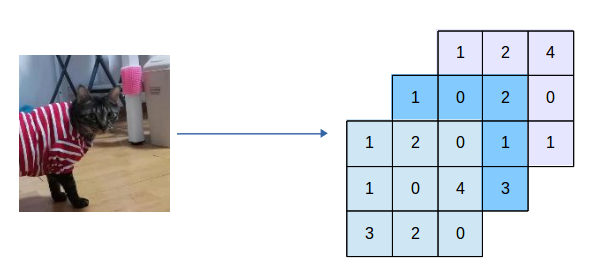
\includegraphics{img/ch5/Image-process.png} \textbar{}
卷积神经网络在图像处理领域有非常广泛的应用,这是因为图像数据本身具有的局部完整性非常
\textbar{} \textbar{} 自然语言处理 \textbar{}
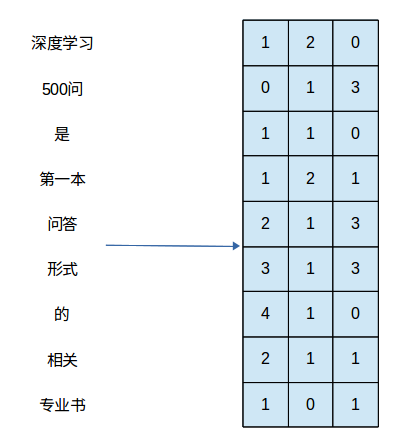
\includegraphics{img/ch5/NLP.png} \textbar{} \textbar{} \textbar{}
语音处理 \textbar{} 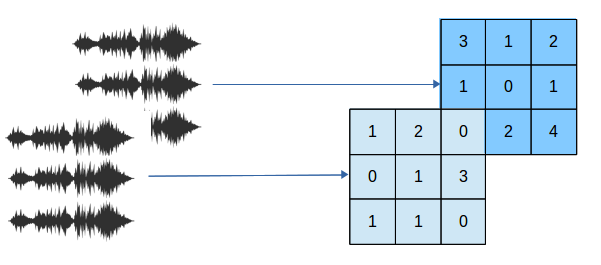
\includegraphics{img/ch5/audio-recognition.png}
\textbar{} \textbar{}

\subsubsection{5.18.1 联系}\label{ux8054ux7cfb}

​ 自然语言处理是对一维信号(词序列)做操作。 ​
计算机视觉是对二维(图像)或三维(视频流)信号做操作。

\subsubsection{5.18.2 区别}\label{ux533aux522b}

​
自然语言处理的输入数据通常是离散取值(例如表示一个单词或字母通常表示为词典中的one
hot向量),计算机视觉则是连续取值(比如归一化到0,1之间的灰度值)。CNN有两个主要特点,区域不变性(location
invariance)和组合性(Compositionality)。

\begin{enumerate}
\def\labelenumi{\arabic{enumi}.}
\tightlist
\item
  区域不变性:滤波器在每层的输入向量(图像)上滑动,检测的是局部信息,然后通过pooling取最大值或均值。pooling这步综合了局部特征,失去了每个特征的位置信息。这很适合基于图像的任务,比如要判断一幅图里有没有猫这种生物,你可能不会去关心这只猫出现在图像的哪个区域。但是在NLP里,词语在句子或是段落里出现的位置,顺序,都是很重要的信息。
\item
  局部组合性:CNN中,每个滤波器都把较低层的局部特征组合生成较高层的更全局化的特征。这在CV里很好理解,像素组合成边缘,边缘生成形状,最后把各种形状组合起来得到复杂的物体表达。在语言里,当然也有类似的组合关系,但是远不如图像来的直接。而且在图像里,相邻像素必须是相关的,相邻的词语却未必相关。
\end{enumerate}

\subsection{5.19
卷积神经网络凸显共性的方法?}\label{ux5377ux79efux795eux7ecfux7f51ux7edcux51f8ux663eux5171ux6027ux7684ux65b9ux6cd5}

\subsubsection{5.19.1 局部连接}\label{ux5c40ux90e8ux8fdeux63a5}

​
我们首先了解一个概念,感受野,即每个神经元仅与输入神经元相连接的一块区域。
在图像卷积操作中,神经元在空间维度上是局部连接,但在深度上是全连接。局部连接的思想,是受启发于生物学里的视觉系统结构,视觉皮层的神经元就是仅用局部接受信息。对于二维图像,局部像素关联性较强。这种局部连接保证了训练后的滤波器能够对局部特征有最强的响应,使神经网络可以提取数据的局部特征;
下图是一个很经典的图示,左边是全连接,右边是局部连接。

\begin{figure}
\centering
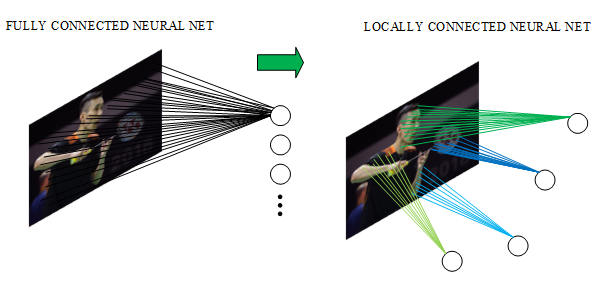
\includegraphics{./img/ch5/5.27.1.png}
\caption{image}
\end{figure}

对于一个1000 ×
1000的输入图像而言,如果下一个隐藏层的神经元数目为10\^{}6个,采用全连接则有1000
× 1000 × 10\^{}6 =
10\^{}12个权值参数,如此巨大的参数量几乎难以训练;而采用局部连接,隐藏层的每个神经元仅与图像中10
× 10的局部图像相连接,那么此时的权值参数数量为10 × 10 × 10\^{}6 =
10\^{}8,将直接减少4个数量级。

\subsubsection{5.19.2 权值共享}\label{ux6743ux503cux5171ux4eab}

​
权值共享,即计算同一深度的神经元时采用的卷积核参数是共享的。权值共享在一定程度上讲是有意义的,是由于在神经网络中,提取的底层边缘特征与其在图中的位置无关。但是在另一些场景中是无意的,如在人脸识别任务,我们期望在不同的位置学到不同的特征。
需要注意的是,权重只是对于同一深度切片的神经元是共享的。在卷积层中,通常采用多组卷积核提取不同的特征,即对应的是不同深度切片的特征,而不同深度切片的神经元权重是不共享。相反,偏置这一权值对于同一深度切片的所有神经元都是共享的。
权值共享带来的好处是大大降低了网络的训练难度。如下图,假设在局部连接中隐藏层的每一个神经元连接的是一个10
× 10的局部图像,因此有10 × 10个权值参数,将这10 ×
10个权值参数共享给剩下的神经元,也就是说隐藏层中10\^{}6个神经元的权值参数相同,那么此时不管隐藏层神经元的数目是多少,需要训练的参数就是这
10 × 10个权值参数(也就是卷积核的大小)。

\begin{figure}
\centering
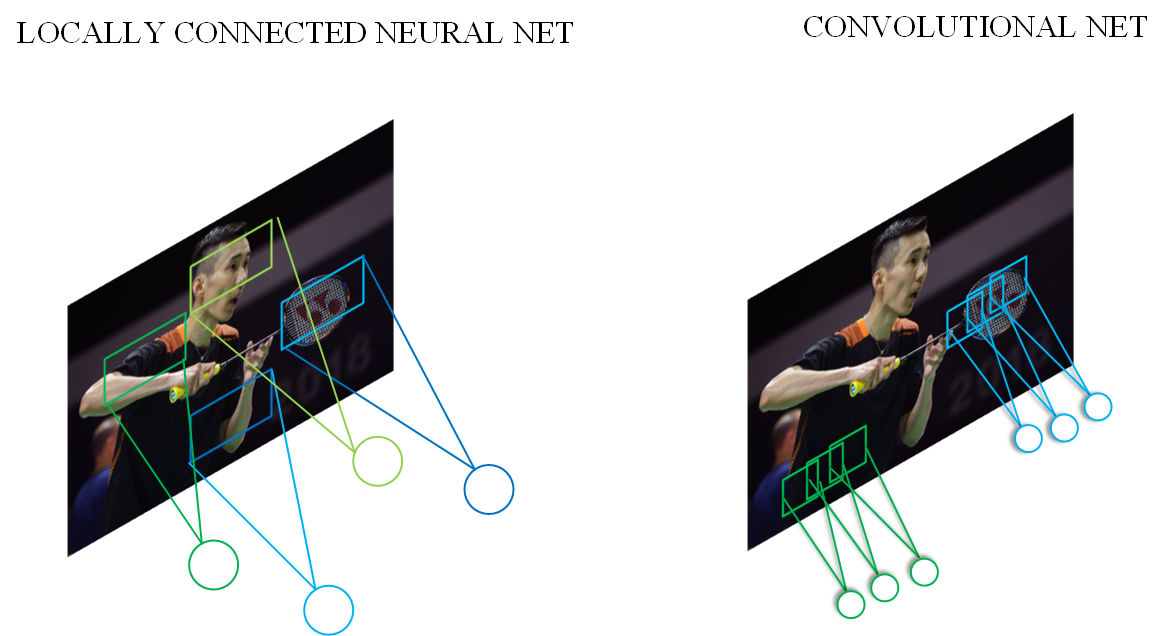
\includegraphics{./img/ch5/5.27.2.png}
\caption{image}
\end{figure}

这里就体现了卷积神经网络的奇妙之处,使用少量的参数,却依然能有非常出色的性能。上述仅仅是提取图像一种特征的过程。如果要多提取出一些特征,可以增加多个卷积核,不同的卷积核能够得到图像不同尺度下的特征,称之为特征图(feature
map)。

\subsubsection{5.19.3 池化操作}\label{ux6c60ux5316ux64cdux4f5c}

池化操作与多层次结构一起,实现了数据的降维,将低层次的局部特征组合成为较高层次的特征,从而对整个图片进行表示。如下图:

\begin{figure}
\centering
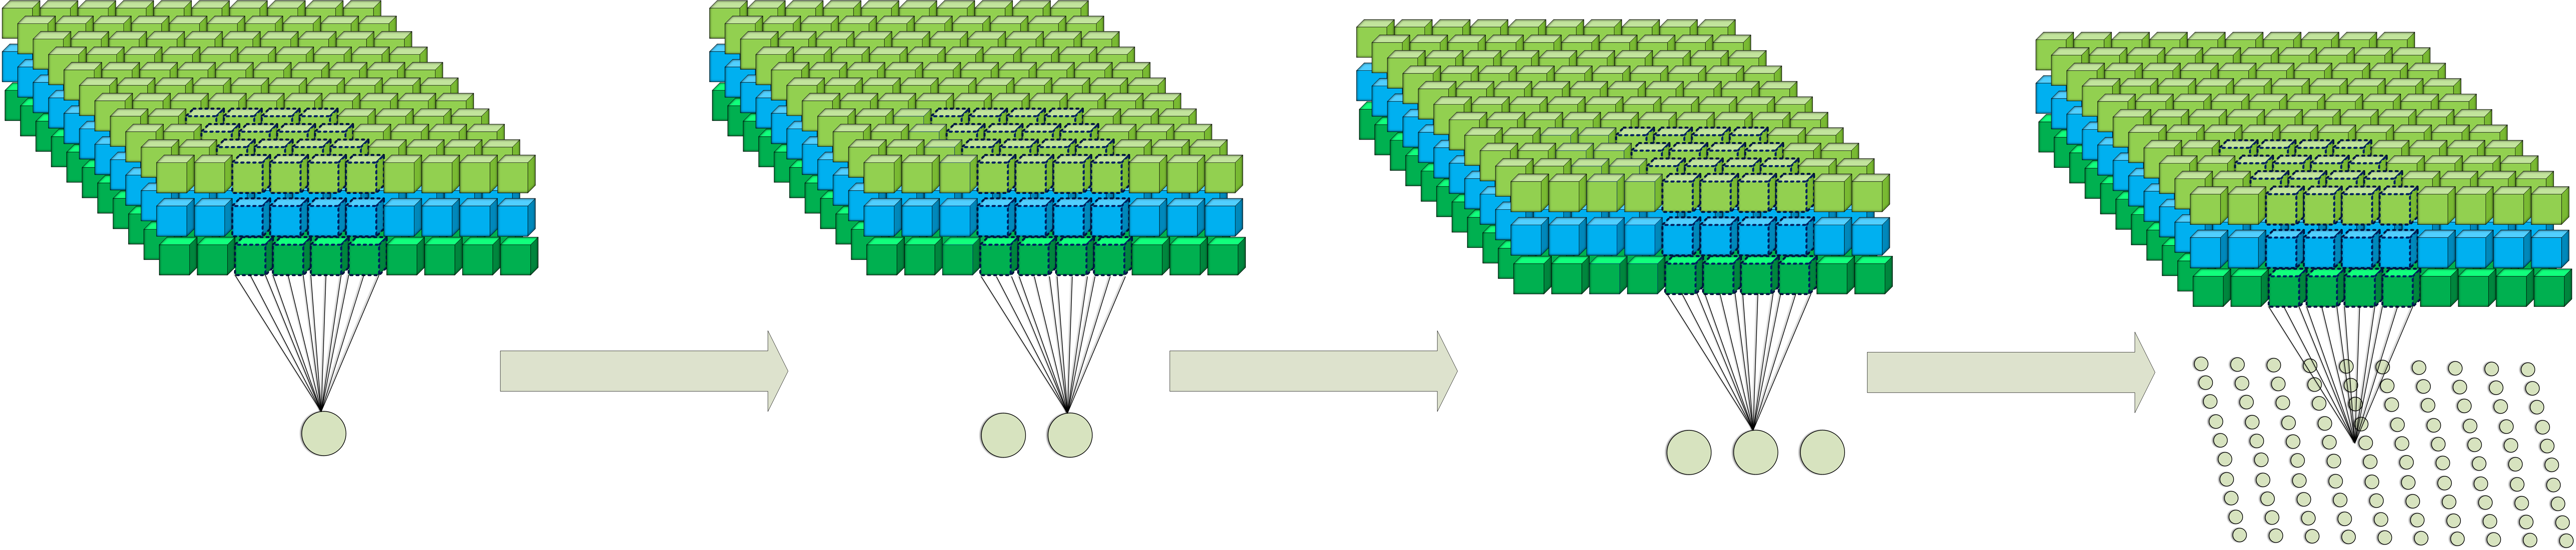
\includegraphics{./img/ch5/5.27.3.png}
\caption{image}
\end{figure}

\subsection{5.20
全连接、局部连接、全卷积与局部卷积}\label{ux5168ux8fdeux63a5ux5c40ux90e8ux8fdeux63a5ux5168ux5377ux79efux4e0eux5c40ux90e8ux5377ux79ef}

​ 大多数神经网络中高层网络通常会采用全连接层(Global Connected
Layer),通过多对多的连接方式对特征进行全局汇总,可以有效地提取全局信息。但是全连接的方式需要大量的参数,是神经网络中最占资源的部分之一,因此就需要由局部连接(Local
Connected
Layer),仅在局部区域范围内产生神经元连接,能够有效地减少参数量。根据卷积操作的作用范围可以分为全卷积(Global
Convolution)和局部卷积(Local
Convolution)。实际上这里所说的全卷积就是标准卷积,即在整个输入特征维度范围内采用相同的卷积核参数进行运算,全局共享参数的连接方式可以使神经元之间的连接参数大大减少;局部卷积又叫平铺卷积(Tiled
Convolution)或非共享卷积(Unshared
Convolution),是局部连接与全卷积的折衷。四者的比较如表XX所示。 ​ 表XX
卷积网络中连接方式的对比

\begin{longtable}[]{@{}ccl@{}}
\toprule
\begin{minipage}[b]{0.11\columnwidth}\centering\strut
连接方式\strut
\end{minipage} & \begin{minipage}[b]{0.08\columnwidth}\centering\strut
示意图\strut
\end{minipage} & \begin{minipage}[b]{0.06\columnwidth}\raggedright\strut
说明\strut
\end{minipage}\tabularnewline
\midrule
\endhead
\begin{minipage}[t]{0.11\columnwidth}\centering\strut
全连接\strut
\end{minipage} & \begin{minipage}[t]{0.08\columnwidth}\centering\strut
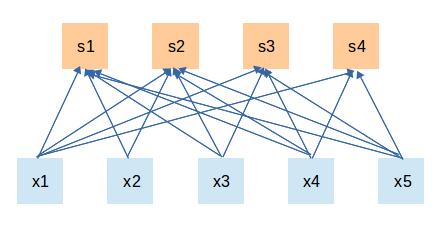
\includegraphics{img/ch5/full-connected.png}\strut
\end{minipage} & \begin{minipage}[t]{0.06\columnwidth}\raggedright\strut
层间神经元完全连接,每个输出神经元可以获取到所有输入神经元的信息,有利于信息汇总,常置于网络末层;连接与连接之间独立参数,大量的连接大大增加模型的参数规模。\strut
\end{minipage}\tabularnewline
\begin{minipage}[t]{0.11\columnwidth}\centering\strut
局部连接\strut
\end{minipage} & \begin{minipage}[t]{0.08\columnwidth}\centering\strut
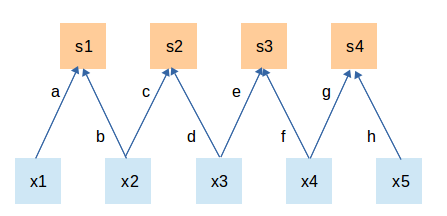
\includegraphics{img/ch5/local-connected.png}\strut
\end{minipage} & \begin{minipage}[t]{0.06\columnwidth}\raggedright\strut
层间神经元只有局部范围内的连接,在这个范围内采用全连接的方式,超过这个范围的神经元则没有连接;连接与连接之间独立参数,相比于全连接减少了感受域外的连接,有效减少参数规模\strut
\end{minipage}\tabularnewline
\begin{minipage}[t]{0.11\columnwidth}\centering\strut
全卷积\strut
\end{minipage} & \begin{minipage}[t]{0.08\columnwidth}\centering\strut
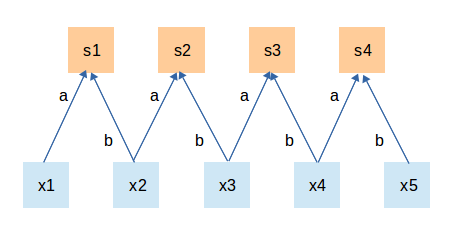
\includegraphics{img/ch5/conv.png}\strut
\end{minipage} & \begin{minipage}[t]{0.06\columnwidth}\raggedright\strut
层间神经元只有局部范围内的连接,在这个范围内采用全连接的方式,连接所采用的参数在不同感受域之间共享,有利于提取特定模式的特征;相比于局部连接,共用感受域之间的参数可以进一步减少参数量。\strut
\end{minipage}\tabularnewline
\begin{minipage}[t]{0.11\columnwidth}\centering\strut
局部卷积\strut
\end{minipage} & \begin{minipage}[t]{0.08\columnwidth}\centering\strut
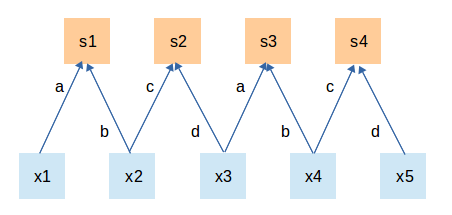
\includegraphics{img/ch5/local-conv.png}\strut
\end{minipage} & \begin{minipage}[t]{0.06\columnwidth}\raggedright\strut
层间神经元只有局部范围内的连接,感受域内采用全连接的方式,而感受域之间间隔采用局部连接与全卷积的连接方式;相比与全卷积成倍引入额外参数,但有更强的灵活性和表达能力;相比于局部连接,可以有效控制参数量\strut
\end{minipage}\tabularnewline
\bottomrule
\end{longtable}

\subsection{5.21
局部卷积的应用}\label{ux5c40ux90e8ux5377ux79efux7684ux5e94ux7528}

并不是所有的卷积都会进行权重共享,在某些特定任务中,会使用不权重共享的卷积。下面通过人脸这一任务来进行讲解。在读人脸方向的一些paper时,会发现很多都会在最后加入一个Local
Connected
Conv,也就是不进行权重共享的卷积层。总的来说,这一步的作用就是使用3D模型来将人脸对齐,从而使CNN发挥最大的效果。
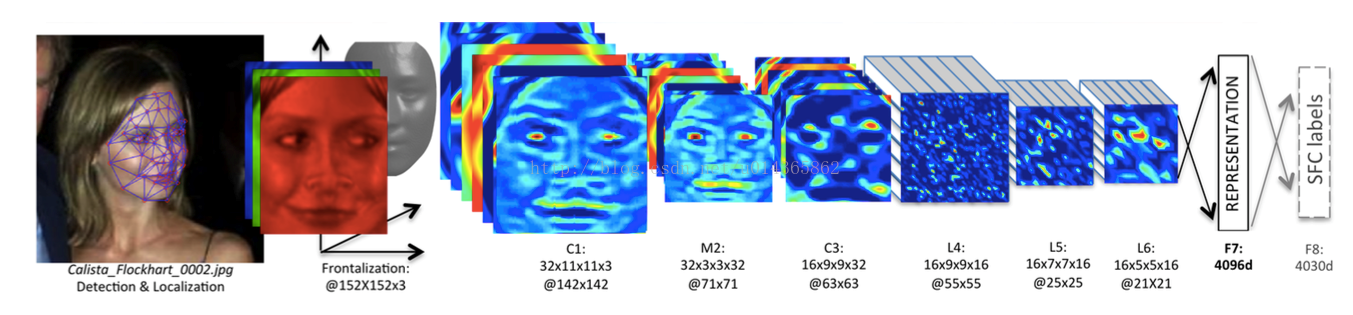
\includegraphics{./img/ch5/img66.png}

截取论文中的一部分图,经过3D对齐以后,形成的图像均是152×152,输入到上述的网络结构中。该结构的参数如下:

Conv:32个11×11×3的卷积核,

Max-pooling: 3×3,stride=2,

Conv: 16个9×9的卷积核,

Local-Conv: 16个9×9的卷积核,

Local-Conv: 16个7×7的卷积核,

Local-Conv: 16个5×5的卷积核,

Fully-connected: 4096维,

Softmax: 4030维。

前三层的目的在于提取低层次的特征,比如简单的边和纹理。其中Max-pooling层使得卷积的输出对微小的偏移情况更加鲁棒。但不能使用更多的Max-pooling层,因为太多的Max-pooling层会使得网络损失图像信息。全连接层将上一层的每个单元和本层的所有单元相连,用来捕捉人脸图像不同位置特征之间的相关性。最后使用softmax层用于人脸分类。
中间三层都是使用参数不共享的卷积核,之所以使用参数不共享,有如下原因:

(1)对齐的人脸图片中,不同的区域会有不同的统计特征,因此并不存在特征的局部稳定性,所以使用相同的卷积核会导致信息的丢失。

(2)不共享的卷积核并不增加inference时特征的计算量,仅会增加训练时的计算量。
使用不共享的卷积核,由于需要训练的参数量大大增加,因此往往需要通过其他方法增加数据量。

\subsection{5.22 NetVLAD池化
(贡献者:熊楚原-中国人民大学)}\label{netvladux6c60ux5316-ux8d21ux732eux8005ux718aux695aux539f-ux4e2dux56fdux4ebaux6c11ux5927ux5b66}

NetVLAD是论文{[}15{]}提出的一个局部特征聚合的方法。

在传统的网络里面,例如VGG啊,最后一层卷积层输出的特征都是类似于Batchsize
x 3 x 3 x 512的这种东西,然后会经过FC聚合,或者进行一个Global Average
Pooling(NIN里的做法),或者怎么样,变成一个向量型的特征,然后进行Softmax
or 其他的Loss。

这种方法说简单点也就是输入一个图片或者什么的结构性数据,然后经过特征提取得到一个长度固定的向量,之后可以用度量的方法去进行后续的操作,比如分类啊,检索啊,相似度对比等等。

那么NetVLAD考虑的主要是最后一层卷积层输出的特征这里,我们不想直接进行欠采样或者全局映射得到特征,对于最后一层输出的W
x H x D,设计一个新的池化,去聚合一个``局部特征``,这即是NetVLAD的作用。

NetVLAD的一个输入是一个W x H x D的图像特征,例如VGG-Net最后的3 x 3 x
512这样的矩阵,在网络中还需加一个维度为Batchsize。

NetVLAD还需要另输入一个标量K即表示VLAD的聚类中心数量,它主要是来构成一个矩阵C,是通过原数据算出来的每一个\(W \times H\)特征的聚类中心,C的shape即\(C: K \times D\),然后根据三个输入,VLAD是计算下式的V:

\[V(j, k) = \sum_{i=1}^{N}{a_k(x_i)(x_i(j) - c_k(j))}\]

其中j表示维度,从1到D,可以看到V的j是和输入与c对应的,对每个类别k,都对所有的x进行了计算,如果\(x_i\)属于当前类别k,\(a_k=1\),否则\(a_k=0\),计算每一个x和它聚类中心的残差,然后把残差加起来,即是每个类别k的结果,最后分别L2正则后拉成一个长向量后再做L2正则,正则非常的重要,因为这样才能统一所有聚类算出来的值,而残差和的目的主要是消减不同聚类上的分布不均,两者共同作用才能得到最后正常的输出。

输入与输出如下图所示:

\begin{figure}
\centering
\includegraphics{http://www.ecohnoch.cn/img/netvlad.jpeg}
\caption{image}
\end{figure}

中间得到的K个D维向量即是对D个x都进行了与聚类中心计算残差和的过程,最终把K个D维向量合起来后进行即得到最终输出的\(K \times D\)长度的一维向量。

而VLAD本身是不可微的,因为上面的a要么是0要么是1,表示要么当前描述x是当前聚类,要么不是,是个离散的,NetVLAD为了能够在深度卷积网络里使用反向传播进行训练,对a进行了修正。

那么问题就是如何重构一个a,使其能够评估当前的这个x和各个聚类的关联程度?用softmax来得到:

\[a_k = \frac{e^{W_k^T x_i + b_k}}{e^{W_{k'}^T x_i + b_{k'}}}\]

将这个把上面的a替换后,即是NetVLAD的公式,可以进行反向传播更新参数。

所以一共有三个可训练参数,上式a中的\(W: K \times D\),上式a中的\(b: K \times 1\),聚类中心\(c: K \times D\),而原始VLAD只有一个参数c。

最终池化得到的输出是一个恒定的K x
D的一维向量(经过了L2正则),如果带Batchsize,输出即为Batchsize x (K x
D)的二维矩阵。

NetVLAD作为池化层嵌入CNN网络即如下图所示,

\begin{figure}
\centering
\includegraphics{http://www.ecohnoch.cn/img/netvlad_emb.png}
\caption{image}
\end{figure}

原论文中采用将传统图像检索方法VLAD进行改进后应用在CNN的池化部分作为一种另类的局部特征池化,在场景检索上取得了很好的效果。

后续相继又提出了ActionVLAD、ghostVLAD等改进。

\subsection{参考文献}\label{ux53c2ux8003ux6587ux732e}

{[}1{]} 卷积神经网络研究综述{[}J{]}. 计算机学报, 2017, 40(6):1229-1251.

{[}2{]} 常亮, 邓小明, 周明全,等. 图像理解中的卷积神经网络{[}J{]}.
自动化学报, 2016, 42(9):1300-1312.

{[}3{]} Chua L O. CNN: A Paradigm for Complexity{[}M{]}// CNN a paradigm
for complexity /. 1998.

{[}4{]} He K, Gkioxari G, Dollar P, et al. Mask R-CNN{[}J{]}. IEEE
Transactions on Pattern Analysis \& Machine Intelligence, 2017,
PP(99):1-1.

{[}5{]} Hoochang S, Roth H R, Gao M, et al. Deep Convolutional Neural
Networks for Computer-Aided Detection: CNN Architectures, Dataset
Characteristics and Transfer Learning{[}J{]}. IEEE Transactions on
Medical Imaging, 2016, 35(5):1285-1298.

{[}6{]} 许可. 卷积神经网络在图像识别上的应用的研究{[}D{]}. 浙江大学,
2012.

{[}7{]} 陈先昌. 基于卷积神经网络的深度学习算法与应用研究{[}D{]}.
浙江工商大学, 2014.

{[}8{]} {[}CS231n Convolutional Neural Networks for Visual Recognition,
Stanford{]}(http://cs231n.github.io/convolutional-networks/)

{[}9{]} {[}Machine Learning is Fun! Part 3: Deep Learning and
Convolutional Neural
Networks{]}(https://medium.com/@ageitgey/machine-learning-is-fun-part-3-deep-learning-and-convolutional-neural-networks-f40359318721\#.2gfx5zcw3)

{[}10{]} cs231n
动态卷积图:\url{http://cs231n.github.io/assets/conv-demo/index.html}

{[}11{]} Krizhevsky A, Sutskever I, Hinton G E. Imagenet classification
with deep convolutional neural networks{[}C{]}//Advances in neural
information processing systems. 2012: 1097-1105.

{[}12{]} Sun Y, Wang X, Tang X. Deep learning face representation from
predicting 10,000 classes{[}C{]}//Computer Vision and Pattern
Recognition (CVPR), 2014 IEEE Conference on. IEEE, 2014: 1891-1898.

{[}13{]}
魏秀参.解析深度学习------卷积神经网络原理与视觉实践{[}M{]}.电子工业出版社,
2018

{[}14{]} Jianxin W U , Gao B B , Wei X S , et al. Resource-constrained
deep learning: challenges and practices{[}J{]}. Scientia
Sinica(Informationis), 2018.

{[}15{]} Arandjelovic R , Gronat P , Torii A , et al. {[}IEEE 2016 IEEE
Conference on Computer Vision and Pattern Recognition (CVPR) - Las
Vegas, NV, USA (2016.6.27-2016.6.30){]} 2016 IEEE Conference on Computer
Vision and Pattern Recognition (CVPR) - NetVLAD: CNN Architecture for
Weakly Supervised Place Recognition{[}C{]}// 2016:5297-5307.
